A command group can contain three different things: an action, its dependences, and miscellaneous host code. Of these three things, the one that is always required is the action since without it, the command group really doesn’t do anything. Most command groups will also express dependences, but there are cases where they may not. One such example is the first action submitted in a program. It does not depend on anything to begin execution; therefore, we would not specify any dependence. The other thing that can appear inside a command group is arbitrary C++ code that executes on the host. This is perfectly legal and can be useful to help specify the action or its dependences, and this code is executed while the command group is created (not later when the action is performed based on dependences having been met).\par

Command groups are typically expressed as a C++ lambda expression passed to the submit method. Command groups can also be expressed through shortcut methods on queue objects that take a kernel and set of event-based dependences.\par

\hspace*{\fill} \par %插入空行
\textbf{Command Group Actions}

There are two types of actions that may be performed by a command group: kernels and explicit memory operations. A command group may only perform a single action. As we’ve seen in earlier chapters, kernels are defined through calls to a parallel\_for or single\_task method and express computations that we want to perform on our devices. Operations for explicit data movement are the second type of action. Examples from USM include memcpy, memset, and fill operations. Examples from buffers include copy, fill, and update\_host.\par

\hspace*{\fill} \par %插入空行
\textbf{How Command Groups Declare Dependences}

The other main component of a command group is the set of dependences that must be satisfied before the action defined by the group can execute. DPC++ allows these dependences to be specified in several ways.\par

If a program uses in-order DPC++ queues, the in-order semantics of the queue specify implicit dependences between successively enqueued command groups. One task cannot execute until the previously submitted task has completed.\par

Event-based dependences are another way to specify what must be complete before a command group may execute. These event-based dependences may be specified in two ways. The first way is used when a command group is specified as a lambda passed to a queue’s submit method. In this case, the programmer invokes the depends\_on method of the command group handler object, passing either an event or vector of events as parameter. The other way is used when a command group is created from the shortcut methods defined on the queue object. When the programmer directly invokes parallel\_for or single\_task on a queue, an event or vector of events may be passed as an extra parameter.\par

The last way that dependences may be specified is through the creation of accessor objects. Accessors specify how they will be used to read or write data in a buffer object, letting the runtime use this information to determine the data dependences that exist between different kernels. As we reviewed in the beginning of this chapter, examples of data dependences include one kernel reading data that another produces, two kernels writing the same data, or one kernel modifying data after another kernel reads it.\par

\hspace*{\fill} \par %插入空行
\textbf{Examples}

Now we will illustrate everything we’ve just learned with several examples. We will present how one might express two different dependence patterns in several ways. The two patterns we will illustrate are linear dependence chains where one task executes after another and a “Y” pattern where two independent tasks must execute before successive tasks.\par

Graphs for these dependence patterns can be seen in Figures 8-1 and 8-2. Figure 8-1 depicts a linear dependence chain. The first node represents the initialization of data, while the second node presents the reduction operation that will accumulate the data into a single result. Figure 8-2 depicts a “Y” pattern where we independently initialize two different pieces of data. After the data is initialized, an addition kernel will sum the two vectors together. Finally, the last node in the graph accumulates the result into a single value.\par

\hspace*{\fill} \par %插入空行
Figure 8-1. Linear dependence chain graph
\begin{center}
	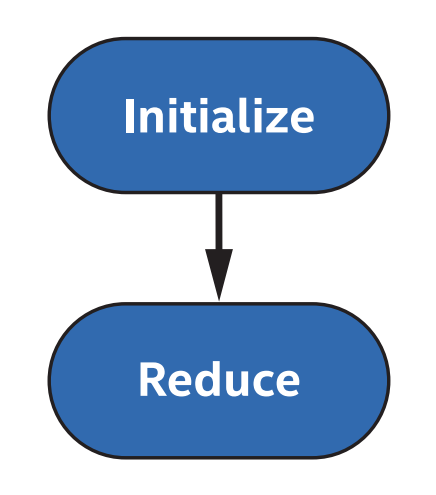
\includegraphics[width=0.2\textwidth]{content/chapter-8/images/2}
\end{center}

For each pattern, we will show three different implementations. The first implementation will use in-order queues. The second will use event-based dependences. The last implementation will use buffers and accessors to express data dependences between command groups.\par

\hspace*{\fill} \par %插入空行
Figure 8-2. “Y” pattern dependence graph
\begin{center}
	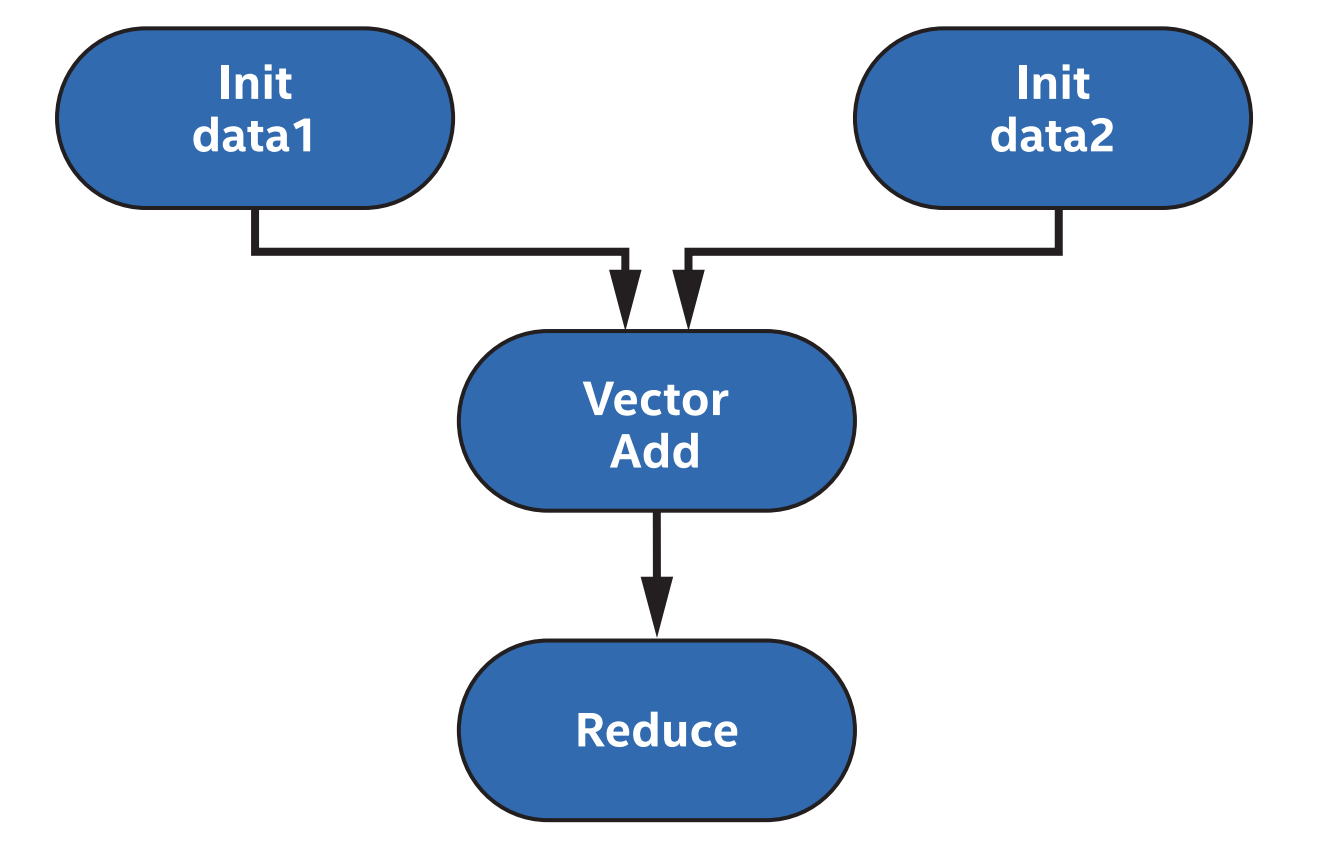
\includegraphics[width=0.5\textwidth]{content/chapter-8/images/3}
\end{center}

\hspace*{\fill} \par %插入空行
Figure 8-3. Linear dependence chain with in-order queues
\begin{lstlisting}[caption={}]
constexpr int N = 42;

queue Q{property::queue::in_order()};

int *data = malloc_shared<int>(N, Q);

Q.parallel_for(N, [=](id<1> i) { data[i] = 1; });

Q.single_task([=]() {
	for (int i = 1; i < N; i++)
		data[0] += data[i];
});

Q.wait();

assert(data[0] == N);
\end{lstlisting}

Figure 8-3 shows how to express a linear dependence chain using in-order queues. This example is very simple because the semantics of inorder queues already guarantee a sequential order of execution between command groups. The first kernel we submit initializes the elements of an array to 1. The next kernel then takes those elements and sums them together into the first element. Since our queue is in order, we do not need to do anything else to express that the second kernel should not execute until the first kernel has completed. Finally, we wait for the queue to finish executing all its tasks, and we check that we obtained the expected result.\par

\hspace*{\fill} \par %插入空行
Figure 8-4. Linear dependence chain with events
\begin{lstlisting}[caption={}]
constexpr int N = 42;

queue Q;

int *data = malloc_shared<int>(N, Q);

auto e = Q.parallel_for(N, [=](id<1> i) { data[i] = 1; });

Q.submit([&](handler &h) {
	h.depends_on(e);
	h.single_task([=]() {
		for (int i = 1; i < N; i++)
			data[0] += data[i];
	});
});

Q.wait();
assert(data[0] == N);
\end{lstlisting}

Figure 8-4 shows the same example using an out-of-order queue and event-based dependences. Here, we capture the event returned by the first call to parallel\_for. The second kernel is then able to specify a dependence on that event and the kernel execution it represents by passing it as a parameter to depends\_on. We will see in Figure 8-6 how we could shorten the expression of the second kernel using one of the shortcut methods for defining kernels.\par

\hspace*{\fill} \par %插入空行
Figure 8-5. Linear dependence chain with buffers and accessors
\begin{lstlisting}[caption={}]
constexpr int N = 42;
queue Q;

buffer<int> data{range{N}};

Q.submit([&](handler &h) {
	accessor a{data, h};
	h.parallel_for(N, [=](id<1> i) { a[i] = 1; });
});

Q.submit([&](handler &h) {
	accessor a{data, h};
	h.single_task([=]() {
		for (int i = 1; i < N; i++)
			a[0] += a[i];
	});
});

host_accessor h_a{data};
assert(h_a[0] == N);
\end{lstlisting}

Figure 8-5 rewrites our linear dependence chain example using buffers and accessors instead of USM pointers. Here we once again use an outof-order queue but use data dependences specified through accessors instead of event-based dependences to order the execution of the command groups. The second kernel reads the data produced by the first kernel, and the runtime can see this because we declare accessors based on the same underlying buffer object. Unlike the previous examples, we do not wait for the queue to finish executing all its tasks. Instead, we declare a host accessor that defines a data dependence between the output of the second kernel and our assertion that we computed the correct answer on the host. Note that while a host accessor gives us an up-to-date view of data on the host, it does not guarantee that the original host memory has been updated if any was specified when the buffer was created. We can’t safely access the original host memory unless the buffer is first destroyed or unless we use a more advanced mechanism like the mutex mechanism described in Chapter 7.\par

\hspace*{\fill} \par %插入空行
Figure 8-6. “Y” pattern with in-order queues
\begin{lstlisting}[caption={}]
constexpr int N = 42;

queue Q{property::queue::in_order()};

int *data1 = malloc_shared<int>(N, Q);
int *data2 = malloc_shared<int>(N, Q);

Q.parallel_for(N, [=](id<1> i) { data1[i] = 1; });

Q.parallel_for(N, [=](id<1> i) { data2[i] = 2; });

Q.parallel_for(N, [=](id<1> i) { data1[i] += data2[i]; });

Q.single_task([=]() {
	for (int i = 1; i < N; i++)
		data1[0] += data1[i];
	data1[0] /= 3;
});

Q.wait();
assert(data1[0] == N);
\end{lstlisting}

Figure 8-6 shows how to express a “Y” pattern using in-order queues. In this example, we declare two arrays, data1 and data2. We then define two kernels that will each initialize one of the arrays. These kernels do not depend on each other, but because the queue is in order, the kernels must execute one after the other. Note that it would be perfectly legal to swap the order of these two kernels in this example. After the second kernel has executed, the third kernel adds the elements of the second array to those of the first array. The final kernel sums up the elements of the first array to compute the same result we did in our examples for linear dependence chains. This summation kernel depends on the previous kernel, but this linear chain is also captured by the in-order queue. Finally, we wait for all kernels to complete and validate that we successfully computed our magic number.\par

\hspace*{\fill} \par %插入空行
Figure 8-7. “Y” pattern with events
\begin{lstlisting}[caption={}]
constexpr int N = 42;
queue Q;

int *data1 = malloc_shared<int>(N, Q);
int *data2 = malloc_shared<int>(N, Q);

auto e1 = Q.parallel_for(N, 
			[=](id<1> i) { data1[i] = 1; });

auto e2 = Q.parallel_for(N, 
			[=](id<1> i) { data2[i] = 2; });

auto e3 = Q.parallel_for(range{N}, {e1, e2},
			[=](id<1> i) { data1[i] += data2[i]; });
	
Q.single_task(e3, [=]() {
	for (int i = 1; i < N; i++)
		data1[0] += data1[i];
	data1[0] /= 3;
});

Q.wait();
assert(data1[0] == N);
\end{lstlisting}

Figure 8-7 shows our “Y” pattern example with out-of-order queues instead of in-order queues. Since the dependences are no longer implicit due to the order of the queue, we must explicitly specify the dependences between command groups using events. As in Figure 8-6, we begin by defining two independent kernels that have no initial dependences. We represent these kernels by two events, e1 and e2. When we define our third kernel, we must specify that it depends on the first two kernels. We do this by saying that it depends on events e1 and e2 to complete before it may execute. However, in this example, we use a shortcut form to specify these dependences instead of the handler’s depends\_on method. Here, we pass the events as an extra parameter to parallel\_for. Since we want to pass multiple events at once, we use the form that accepts a std::vector of events, but luckily modern C++ simplifies this for us by automatically converting the expression {e1, e2} into the appropriate vector.\par

\hspace*{\fill} \par %插入空行
Figure 8-8. “Y” pattern with accessors
\begin{lstlisting}[caption={}]
constexpr int N = 42;
queue Q;

buffer<int> data1{range{N}};
buffer<int> data2{range{N}};

Q.submit([&](handler &h) {
	accessor a{data1, h};
	h.parallel_for(N, [=](id<1> i) { a[i] = 1; });
});

Q.submit([&](handler &h) {
	accessor b{data2, h};
	h.parallel_for(N, [=](id<1> i) { b[i] = 2; });
});

Q.submit([&](handler &h) {
	accessor a{data1, h};
	accessor b{data2, h, read_only};
	h.parallel_for(N, [=](id<1> i) { a[i] += b[i]; });
});

Q.submit([&](handler &h) {
	accessor a{data1, h};
	h.single_task([=]() {
		for (int i = 1; i < N; i++)
			a[0] += a[i];
		a[0] /= 3;
	});
});

host_accessor h_a{data1};
assert(h_a[0] == N);
\end{lstlisting}

In our final example, seen in Figure 8-8, we again replace USM pointers and events with buffers and accessors. This example represents the two arrays data1 and data2 as buffer objects. Our kernels no longer use the shortcut methods for defining kernels since we must associate accessors with a command group handler. Once again, the third kernel must capture the dependence on the first two kernels. Here this is accomplished by declaring accessors for our buffers. Since we have previously declared accessors for these buffers, the runtime is able to properly order the execution of these kernels. Additionally, we also provide extra information to the runtime here when we declare accessor b. We add the access tag read\_only to let the runtime know that we’re only going to read this data, not produce new values. As we saw in our buffer and accessor example for linear dependence chains, our final kernel orders itself by updating the values produced in the third kernel. We retrieve the final value of our computation by declaring a host accessor that will wait for the final kernel to finish executing before moving the data back to the host where we can read it and assert we computed the correct result.\par 

\hspace*{\fill} \par %插入空行
\textbf{When Are the Parts of a CG Executed?}

Since task graphs are asynchronous, it makes sense to wonder when exactly command groups are executed. By now, it should be clear that kernels may be executed as soon as their dependences have been satisfied, but what happens with the host portion of a command group?\par

When a command group is submitted to a queue, it is executed immediately on the host (before the submit call returns). This host portion of the command group is executed only once. Any kernel or explicit data operation defined in the command group is enqueued for execution on the device.\par

































